\documentclass[a4paper, 11pt, titlepage]{article}
\usepackage{a4wide}
\usepackage{amsmath}

\usepackage[pdftex]{graphicx}
\usepackage{pdfpages}
\usepackage{subcaption}
\usepackage{listings}
\usepackage{color}
\usepackage{cite}
\usepackage{import}
\usepackage[title,titletoc,toc]{appendix}


\newcommand{\HRule}{\rule{\linewidth}{0.5mm}}

%Colours!
%\usepackage[table]{xcolor}
\definecolor{mygreen}{rgb}{0,0.6,0}
\definecolor{mygray}{rgb}{0.5,0.5,0.5}
\definecolor{mymauve}{rgb}{0.58,0,0.82}
\definecolor{mynavyblue}{HTML}{1E5A9C}

%PDF hyperlinks
\usepackage{hyperref}
\hypersetup{
     colorlinks   = true,
     citecolor    = black,
     linkcolor    = black,
     urlcolor   = mynavyblue,
     bookmarksopen  = false,
     pdfpagemode  = UseNone,
     pdftitle   = {Hexacopter Project 2015},
     pdfauthor    = {},
     pdfsubject = {Hexacopter FYP 2015}
}



\begin{document}


  
\begin{titlepage}
\begin{center}

% Upper part of the page. The '~' is needed because \\
% only works if a paragraph has started.

\includegraphics[width=0.7\textwidth]{./logo.png}~\\[1cm]

\textsc{\Large Final Year Project Proposal}\\[0.5cm]

% Title
\HRule \\[0.4cm]
{ \huge \bfseries Towards Autonomous Search and Discovery in UAVs \\[0.4cm] }

\HRule \\[1.5cm]

% Author and supervisor
\noindent
\begin{minipage}[t]{0.4\textwidth}
\begin{flushleft} \large
\emph{Author:}\\
Brett \textsc{Downing}
\end{flushleft}
\end{minipage}%
\begin{minipage}[t]{0.4\textwidth}
\begin{flushright} \large
\emph{Supervisors:} \\
Prof.~Thomas \textsc{Braunl}\\
Chris \textsc{Croft}
\end{flushright}
\end{minipage}

\vfill

% Bottom of the page
{\large \today}

\end{center}
\end{titlepage}

  %\maketitle
  \begin{abstract}
  Multirotors are here to stay, and may soon be expected to interact in a human environment.
  Commodity quadcopters are advertising capabilities to act as  chase-cams and turn-key mapping solutions, but none of the current generation commodity uav chase-cams offer computer vision driven or even assisted flight modes to improve tracking, image framing or obstacle avoidance.  Such vision assisted routines would also apply to autonomous or semi-autonomous inspection tasks for fixtures in remote or hazardous environments.

  In this project, we build on the results of previous year groups and implement turn-key waypoint navigation and failsafe methods using the ardupilot software stack, and develop robust object tracking, data collection behaviours and exclusion zones on a computationally starved platform with an aim to integrate vision assisted behaviours in low-cost, lightweight UAVs.
  \end{abstract}

  \tableofcontents
  \pagebreak
  \section{Introduction}
    Background, Aims

    \subsection{Motivation}
      Recent Developments in power and control electronics has allowed small, consumer level UAVs to lift enough processing capacity to navigate at least partly by computer vision.

      A number of Commercial Micro UAVs are beginning to advertise the ability to act as an autonomous chase-cam \cite{Lily} \cite{AirDog}.  Almost all of these systems rely on a tracking device on the user, and many navigate entirely by GPS.  While the performance of GPS is improving, the performance of a chase-cam will be limited to the update rate and fix accuracy of the beacon and drone GPS modules.  It also requires a lock to be achieved in both devices before tracking can commence.

      The power distribution and plant monitoring sectors have recently been taking on small fleets of drones to perform routine inspection of remote, hazardous or otherwise difficult locations \cite{RopeAccess}.  Many of these applications are reasonably repetitive and well defined enough to fully automate, but cannot be navigated by GPS alone due to the poor repeatability of the GPS system.
      During this project, we were approached by a mining safety startup interested in using UAVs for routine site inspections.

      The UAVs we are targeting operate with small payloads, must react quickly to changes in the environment, and frequently feature camera systems.
      Despite falling costs of hobby and toy grade multirotor systems, Collision avoidance, Object tracking,   mapping and inspection are not well catered for in the current market of UAVs.
      Part of the problem is that very few sensors are of the appropriate scale, or mass for low cost UAVs.
      Ground based vehicles have an advantage that a 1D sensor need only be swept in one axis to search for obstacles, but a UAV must collect data filling a volume ahead of it. About the only form of sensor capable of doing this is a 3D laser scanner which is a high-precision, high-cost, high-mass device.
      A simple camera collects data from an appropriately large volume at high enough speeds to navigate a multirotor, but the data is often difficult or computationally expensive to interpret.

      With environmental data collected by an efficient computer-vision routine, the current generation of multi-rotor devices would be able to interact in a human environment.

      Computer vision assisted control routines would permit common low cost UAVs to better frame extreme sport chase-cam film reels, automatically avoid obstacles, and stabilise GPS variances in remotely operated inspection tasks.

      In this study we investigate the usability of computer vision alone to track and follow a moving target.  It is hoped that this work can be used to improve the performance of camera tracking routines in autonomous chase-cam and cinematographic applications, and partially automate remote inspection 

      Much of the technology related to multi-copters is applicable to most other forms of UAV.  The vast array of applications micro UAVs have found suggests this work may find use in Agriculture, mapping, targeted crop dusting, Cinematography, extreme-sport photography, Data collection, remote observation and inspection and hazard and environmental monitoring.

  \section{Background}

    \subsection{Optical Search}
      Search and Rescue is a field that is extremely appropriate to automation due to the difficulty in mobilising teams in remote, harsh or dangerous conditions.  A micro UAV can be deployed quickly and commence the search operation before boots can be placed on the ground.
      The UAV Outback Challenge \cite{OutbackChallenge} is a regular competition to perform various search and rescue missions autonomously.  The performance criteria are deliberately set very high, and the competition frequently goes uncompleted.  
      In 2012, CanberraUAV \cite{canberrauav}, a UAV development team from Canberra completed the search aspect of the competition.
      After trying a number of image recognition algorithms, the search algorithm that they flew with simply looked for the blue of the jeans of Outback Joe \cite{tridge}. This was sufficient to locate the target in a 4x6 km area.  This goes to show that even a minimally complex routine can be effectively applied in appropriate conditions.

    \subsection{Terrain Estimation via Optical Flow Methods}
      Adding sensors to allow the copter to understand its environment is a surprisingly difficult task.  Conventional contact methods operate at ranges far too close for UAVs, ultrasonics are buffeted by down-wash and most depth sensors are either too heavy or suffer under intense light.
      In terms of simplicity of algorithms, biomimicry has turned up some surprising results.  In 2004, a French research group applied a number of optical flow algorithms to the navigation of a small helicopter inspired by insect vision \cite{InsectFlowMethods}.  The computer vision routines were used to inform the navigation loops, following the middle of urban tunnels and reducing speed in dense clutter, without necessarily computing the distance to the obstacles.  These routines were relatively expensive in terms of computational power, but extremely simple and parallelizeable.

    \subsection{Position Estimation using Stereoscopic Methods}
      Any measurement will have an associated uncertainty, extracting the most information out of a collection of measurements rarely involves taking the most accurate measurements.  It is possible to estimate the position of an object or feature using multiple images separated in either space or time, but making effective use the information requires an understanding of how the uncertainties behave.  Error Modeling in Stereo Navigation \cite{stereoUnc} investigates a number of routines to estimate the position of a vehicle by tracking visible land-marks in a stereoscopic system, and notes the interaction between the geometry of the uncertainties, and the stability of the result.

    \subsection{Altitude Estimation and Odometry by optical flow}
      Elementary methods are still interesting for the sake of biomimicry, and indeed, a 20 element photo-array was demonstrated sufficient to control the altitude of an aircraft \cite{optoAlt}, coupling the altitude to the velocity.
      Dedicated, low resolution optical flow sensors have become exceedingly cheap since the market saturation of the optical mouse, and many commodity flight computers already include doppler information from GPS modules. 
      Combining this data allows the UAV to estimate the distance to the terrain, \cite{RemTerrain}.  These commodity sensors typically do not include circuitry for computing rotation, but given the cost of the sensors, that limitation can be overcome using two sensors \cite{FlowRot}.
      With the availability of these parts, a number of UAV systems such as ArduPilot already include support for these devices in their code-base \cite{ArduFlow}.
      This support also covers pitch and roll compensation and position stabilisation using odometetry.


\section{Project History}

    \subsubsection{2013}
      The 2013 team, O'Connor \cite{OConnor} and Venables \cite{Venables} established the project with the purchase of a DJI flame-wheel F550 Hexacopter with a NAZA-lite flight controller.  This copter was fitted and tested, and finally converted into an autonomous platform with the addition of a Raspberry Pi single-board computer (RPi) and a circuit to switch the control channels from the radio receiver to the RPi GPIO outputs.
      The NAZA-lite at this time did not feature telemetry outputs or way-point inputs, but it was able to loiter in a stiff wind using a GPS fix.
      This team gathered location information for the RPi using a Qstarz GPS unit, and bearing information using an X-sens IMU.  The sensor duplication did not exceed the maximum payload capacity of the platform, but it did suffer a short flight-time.
      Under direct control from the RPi, the drone was able to execute basic way-point navigation.
    \subsubsection{2014}

      The 2014 team, Baxter \cite{Baxter}, Mazur \cite{Mazur} and Targhagh \cite{Targhagh} continued the project adding an internet accessible web UI to control the various autonomous features of the platform, displaying the flight-path of the copter and a live feed of the camera.
      The navigation routines were improved and extended to permit operation without reliable heading information, and the computer vision routines were extented.

    \subsubsection{2015}
      The project is being continued by Allen \cite{Allen}, Mohanty \cite{Mohanty}, Tan \cite{Tan} and Downing \cite{Downing}.
      Because of the rapid pace that the market is adopting new features and technologies, we saw fit to undertake a critical review of all aspects of the platform, and begin improvements that facilitate the current typical feature set.


  \subsection{Platform}
    \subsubsection{Description}
      This project centred around a hexacopter based on the DJI F550 frame. This frame allows for a generous lift capacity, and plenty of space to fasten flight assist hardware, and represents a low cost platform so that our work can be reproduced by a sufficiently motivated hobbyist.
      
      In this work, the flight tasks are based around two physically separate processors; the Flight Controller, and the Server. This allows a stable, known safe build to be maintained on the flight controller, while experimental code runs on the server. If the server fails for any reason, the flight controller will maintain flight, and it allows the operator to engage various fail-safe behaviours without having to rely on the experimental code.
      At hand-over, the server was a Raspberry Pi model B+, and the fight controller was a NAZA lite.
      This combination did not go together smoothly. The NAZA lite was designed as an entry level free-flight controller and did not expose any interfaces for telemetry or data acquisition.  As such, the previous teams had to duplicate the GPS and IMU sensors to have that data available to the server's algorithms. 

      The NAZA also did not feature waypoint navigation features, or secondary command channels so the previous teams used a relay board to physically switch the control inputs from the RC receiver to the server, and implemented their own flight control algorithms on the server.  We were told that server lock-ups frequently caused the craft to power-dive.
      
      The server has been upgraded to a Raspberry Pi V2 single board computer, which we consider to be a computationally starved platform.  At the time of writing, the Raspberry Pi V2 has less computational power than a smartphone in the \$200 price bracket.

      Flight controller
       processor, gimbal
    \subsubsection{Platform Weaknesses}
      (fitness for purpose etc)
      We made some attempts to break into the data channel between the NAZA flight controller and its GPS module, but the raw GPS and compass data was not particularly useful without the accelerometer and gyro data.  This channel had also been deliberately obfuscated by DJI, making it quite clear that this was beyond the design intent of the flight controller.  A community RC group had reverse engineered this link, and we ported their code to the raspberry pi and removed the Qstar-z GPS unit.
      
      The physical switch of control from the user to the server, and the ongoing development of a control loop meant that RC switch was never configured to surrender the throttle channel, and the server was left without altitude control.  This meant that the server had continuous perturbations from the user who remained responsible for maintaining a fixed altitude by sight alone.

      The NAZA is a robust, if basic free-flight controller, and did not feature telemetry.  The server did not have access to an estimate of remaining flight time, and the user could not retrieve logs in the case of a crash.

      Waypoints were handled on the server despite the NAZA featuring GPS assisted loiter behaviour, and a reliable return-to-launch failsafe feature.  In general, control loops should be as tight as possible and routing them through an entirely separate processor is clearly an unnecessarily long loop.


  \subsection{Team Achievements}
    \subsubsection{Flight Controller}
    After spending some time with the hardware configuration of the previous teams, we prepared a report outlining the weaknesses and proposing a change.
    We swapped the NAZA flight controller out for a 3DR Pixhawk running the Ardupilot 3.3 firmware.  This gave us Waypoints, altitude control, failsafes, telemetry, and a GPS-only driven follow-me mode out of the box.
    The open and configurable flight controller with built-in autonomous and hybrid modes, meant that we could fully surrender control to the autonomous platform, including altitude control.  The built-in mode change behaviours meant that we could relinquish and resume manual control at the remote, or activate fail-safes just as reliably as with the NAZA.
    
    \subsubsection{Telemetry}
    The telemetry link supports the MAVlink protocol, which defines various commands from interrogating the status to setting waypoints, or even setting the instantaneous velocity vector.  This let us keep the high-speed components of the control loops firmly inside the flight controller, and direct it with the lower speed vision tasks.  This also gave us linear control inputs in SI units.

    \subsubsection{Simulation Environment}
    By using a fully-featured open-source flight controller, we also had access to the community developed simulation environment.  The Ardupilot simulator is designed to simulate the behaviour of the flight controller against various hardware configurations and flight styles.  As such, it incorporates a comprehensive inertial model and noise injection to the various sensors.  We were able to compile our tests for our development machines couple them to the simulator over a local TCP socket, and test them against the same version of the flight control firmware as we had uploaded to the physical copter.

    \subsubsection{Sensor Duplication}
    The new configuration allowed us to fully eliminate duplicated hardware, an opportunity to fully re-build the wiring harness, and significantly reduce the weight of the craft, extending the flight time to almost twenty minutes.
    Near the end of the project, we fitted a second GPS module to the copter to combat the poor multipath environment of the UWA campus.  With the sensor fusion and Extended Kalman Filter in the Ardupilot firmware, we we able to fly on GPS alone in some of the worst urban canyons in the campus.

    (image: GPS track, glitch from Uni Club to Eng Carpark)

    \subsubsection{Web UI}
    We saw fit to refresh the Web UI and HUD, implementing a more appealing and maintainable template system, and adding more information to the display.

    \subsubsection{Cooperative Projects}
    Integration of our projects

    Glyph detection

    Computer vision driven chase-cam behaviour

    Waypoint modifier routine using polygonal no-fly zones and geo-fencing

    Capture and tagging of images to suit proprietary offline 3D reconstruction algorithms.

\section{Object tracker}

  \subsection{Position estimation}
    After experimenting with the rudimentary PID loop, we moved on to basic triangulation methods to estimate the location of the object with the assumption that it was on the ground.  We were estimating the height based on the GPS altitude data streaming from the NAZA GPS, but without access to the NAZA's internal barometer, the uncertainty in height caused the navigation loop stability to vary significantly minute by minute.
    After the upgrade to the Pixhawk, we had access to the data from the Extended Kalman Filter in the flight controller.  We had also made significant changes to the way the flight controller was guided by the server, and this prompted a near total re-write of the object tracking code-base.

  \subsection{Desired relative pose}
    Once the object is located in 3D space, the copter will calculate a vantage point from which to view it.
    This vantage point could include information regarding the terrain, the size and trajectory of the object, the field of view of the camera, locations of light sources etc.  This is the point at which cinematographic style is included in the algorithm.

  \subsection{Motion Control}
    As of version 3.3, The Arducopter code-base has support for arbitrary velocity vectors.  The first iteration of the motion control algorithm mirrored the old PID code base and transmitted a velocity vector in body coordinates to the flight controller and closed the motion loop through the automation server.  The long feedback loops had problems with delays and required detailed tuning.  The Pixhawk already has this tuning, so the motion control code was replaced by a guided-mode waypoint.  Essentially, the automation server transmits the vantage point and a desired yaw value to the Pixhawk leaving the automation code very simple, the feedback loops very tight and fast, and remove utterly redundant tuning parameters.

    Using the Pixhawk's internal control loops to move the copter has one disadvantage relating to update frequency.  The motion commands are sent over an auxiliary telemetry link

  \subsection{Observations and uncertainties}
    \subsubsection{Structure from image}
      Resolving structure from image is a field unto itself.  In general, the computational load of modelling the environment in three dimensions live is beyond supercomputing clusters that would fit in the mass restrictions of most multi-rotors.  However, Simultaneous Localisation and Mapping (SLAM) systems have optimised components of this field to a vast array of algorithms of varying computational power requirements.
      One of the critical features of a modern SLAM systems is an acknowledgement that every measurement comes with some uncertainty. 
      In many cases, the treatment of uncertainty can be very simple, carrying a one-dimensional confidence value, to the very complex, where every aspect of the measurement is recorded for post-processing where non-linear couplings can be accounted for.

      Some systems are beginning to feature graph-traversal techniques where observations are stored as relative links in a graph, and networks are drawn through those links to optimise against the uncertainty of various aspects of the environment.  These techniques allow the landmarks to be unloaded from memory very easily permitting a small live map, and can approach the detail of full-map covariance methods with a second, less-than-live graph traversal process.

    \subsubsection{Observation to Object Allocation}
      \label{sec:objectAllocation}
      With many observations streaming from the camera simultaneously, the algorithm must decide which observation relates to which object in memory.  We developed and tested several algorithms to differentiate objects and refine uncertainties
      Most of these suffered from the objects' uncertainties falling so low that the probability of intersection between observation and model fell below reasonable thresholds and new object models were generated.  Part of the problem behind this is that our object detection is still based on colour thresholding; this generates objects of significant size which goes against the assumption implicit in the normal distributions.

      Ultimately, for the sake of rapid testing, the algorithm we have flown with deletes and regenerates the objects every cycle unless the object leaves the field of view.  This makes it very clear when the object estimation code is behaving erratically.

  \subsection{Uncertainty Analysis}
    A good uncertainty model encodes everything that is known and nothing of what is unknown.  Good treatment of uncertainties combines knowledge without losing information, or adding assumptions.
    In the case of structure from image, a system that extracts maximal information from a single camera should be automatically capable of full stereoscopy using only the uncertainty analyses that applied to the monocular case.

    \subsubsection{Ellipsoidal models with Covariance Matrices}
      For the sake of computational load, we've assumed the collected data has a three dimensional multivariate Normal distribution.  We use the quadratic form which uses the inverse of the covariance matrix.
      \begin{equation}
      PDF = \frac{1}{\sqrt{(2\pi)^k|\Sigma|}} e^{-\frac{1}{2}\left( \left(x-\mu\right)^T \Sigma^{-1} \left(x-\mu\right) \right)}
      \end{equation}
      where
      \begin{equation}
      \Sigma=\begin{bmatrix}
        \sigma_x^2 & \sigma_{xy} & \sigma_{xz} \\[0.3em]
        \sigma_{yx} & \sigma_y^2 & \sigma_{yz} \\[0.3em]
        \sigma_{zx} & \sigma_{zy} & \sigma_z^2 
      \end{bmatrix}, k=3
      \end{equation}
      %get the justification for the product straight
      This method is particularly convenient because the normal distribution behaves as a probability density function, and the combination of two observations is the normalised product of probability density functions.  The product of two elliptical Normal distributions is also an elliptical normal distribution.

      In order to save on computing resources, we use the inverse of the covariance matrix natively \(C\), and ignore the normalisation constant, which has a closed form solution and can be calculated from the inverse covariance matrix directly as follows:
      \begin{equation}
      \frac{\sqrt{|C|}}{\sqrt{(2\pi)^3}}
      \end{equation}
      This allows a slightly faster rasterisation of the probability density than covariance matrices, but more importantly, follows almost exactly the definition of an ellipsoid and permits highly efficient geometric manipulation:
      \begin{equation}
      1 = \left(x-x_0\right)^T A \left(x-x_0\right)
      \end{equation}

      With no normalisation constant, the distribution always has a value of exactly one at the centroid.
      By permitting singular matrices, the ellipsoidal format has the flexibility to represent uncertainty distributions unbounded in length in any direction, representing rays and planes.  These singular forms still combine efficiently to form non-singular localised distributions.
      
    \subsubsection{Transformations}
      These covariance structures are well suited for use as vectors, automatically calculating the uncertainty of any combination of vectors.
      
      Mean:
      Multiple observations of a single point are generally subject to averaging, but assigning weights to superior measurements is often difficult as is a common point of discussion in Kalman Filter design.
      
      If the subject of the measurements is known to be the same object, the object is likely to be at the centroid of the product of the probability density functions.  This takes measurement accuracy into account.
      Using the form above, the product of density functions becomes the sum of polynomials.
      \begin{figure}
      \centering
      \begin{subfigure}{.3\textwidth}
        \centering
        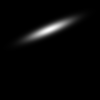
\includegraphics[width=.8\linewidth]{images/GaussianLine1.png}
        \caption{Measurement 1}
        \label{fig:uncProdsub1}
      \end{subfigure}%
      \begin{subfigure}{.3\textwidth}
        \centering
        
\includegraphics[width=.8\linewidth]{images/GaussianLine2.png}
        \caption{Measurement 2}
        \label{fig:uncProdsub2}
      \end{subfigure}
      \begin{subfigure}{.3\textwidth}
        \centering
        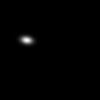
\includegraphics[width=.8\linewidth]{images/GaussianLine3.png}
        \caption{Combined Measurements}
        \label{fig:uncProdsub3}
      \end{subfigure}
      \caption{The Product of Two Measurement Ellipsoids}
      \label{fig:uncProd}
      \end{figure}

      \begin{equation}
      C_3 = C_1+C_2
      \end{equation}
      \begin{equation}
      \mu_3 = C_3^{-1} . (C_1.\mu_1 + C_2.\mu_2)
      \end{equation}
      Clearly apparent here, is that \(\mu_3\) is undefined if \(C_3\) is singular.
      This is not a loss of generality, merely an artefact of the matrix form.  If the matrix \(C_3\) represents a ray, \(C_3\)  will have one eigenvalue of zero and \(\mu\) will have a degree of freedom along the corresponding eigenvector.
      %weak assertion
      In the case of spherical distributions, the successive combination of \(n\) measurements, each with an assumed variance of \(\sigma^2\), will have a resultant variance of \(\sigma^2/n\) which is consistent with treatment of uncertainties in the one dimensional case.
      
      This method minimises the sum of the squares of the Mahalanobis distances between the two ellipsoids, effectively creating a least sum of squares regression method that accounts for the covariance geometry of each measurement as successive ellipsoids are added to the mix.

      Vector sum:
        Treating the ellipsoids as approximate displacement vectors requires the definition of vector operators.
        Again, the matrix form below does not permit singular Matrices as inputs nor outputs, but unpacking it into polynomial form does allow suitable centroids to be chosen.
      \begin{figure}
      \centering
      \begin{subfigure}{.3\textwidth}
        \centering
        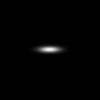
\includegraphics[width=.8\linewidth]{images/GaussianSum1.png}
        \caption{Object at the Origin}
        \label{fig:vectSumsub1}
      \end{subfigure}%
      \begin{subfigure}{.3\textwidth}
        \centering
        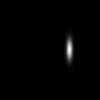
\includegraphics[width=.8\linewidth]{images/GaussianSum2.png}
        \caption{Uncertain Displacement}
        \label{fig:vectSumsub2}
      \end{subfigure}
      \begin{subfigure}{.3\textwidth}
        \centering
        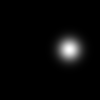
\includegraphics[width=.8\linewidth]{images/GaussianSum3.png}
        \caption{Final Object Location}
        \label{fig:vectSumsub3}
      \end{subfigure}
      \caption{The Vector Sum of Two Uncertainty Distributions}
      \label{fig:vectSum}
      \end{figure}
      \begin{equation}
      C_3 = (C_1^{-1} + C_2^{-1})^{-1}
      \end{equation}
      \begin{equation}
      \mu_3 = \mu_1 + \mu_2
      \end{equation}
      In the same way as above, the vector difference can be computed.  This allows the definition of a discreet time derivative.  A positional derivative defined in this way has an appropriately large velocity uncertainty distribution that increases in size with shorter time-steps, but can be averaged with multiple samples.

      Scale:
      \begin{equation}
      C' = S^{-2} C
      \end{equation}
      \begin{equation}
      \mu' = S \mu
      \end{equation}

      \begin{equation}
      S=\begin{bmatrix}
        S_x & 0 & 0 \\[0.3em]
        0 & S_y & 0 \\[0.3em]
        0 & 0 & S_z
      \end{bmatrix}
      \end{equation}
      Where \(S_n\) represent the change of scale along any axis.


      Rotation:
      The ellipsoidal structure can be rotated as follows:
      \begin{equation}
      C' = R^{-1} C R
      \end{equation}
      \begin{equation}
      \mu' = R^{-1} \mu
      \end{equation}
      Where \(R\) is the rotation matrix.

    \subsubsection{Taking measurements}
      Every sensor on our platform has some resolving power which favours particular directions.
      Our camera cannot locate a point in 3D space, but the direction is known within some small angular uncertainty.
      The Lidar Lite time of flight optical range sensor has a 3 degree conical beam, a 10mm starting aperture, 10mm resolution and a small amount of sample noise. It can locate an object in 3D space, but the uncertainty model favours depth to breadth.
      The GPS gets interesting, In general we can say it has at least 3m sigma = 1 radius. However, over short time periods it has a relative resolution much better than that.
    \subsubsection{The Hyperbolic case}
      \label{sec:hyperbolicCase}
      With a negative determinant, the uncertainty model becomes hyperbolic, expanding to an asymptote with an elliptical conic cross section.  This is interesting because it represents an angular uncertainty, with minimal changes to the uncertainty model.
      In order to represent the hyperbolic distribution, one of the diagonal terms of the covariance matrix must be negative.  Here, positive numbers represent increasing certainty, zero represents total uncertainty.  so mixing a hyperbolic distribution with an elliptical one would suggest that the result contains less information than the elliptical distribution alone.
      This stems from the hyperbola having a normalisation function over its area.  Given that it integrates to infinity, the probability density function would be infinitesimal everywhere.  A more useful description of its behaviour would be that its cross-section integrates to one.
      This model is similar to the definition of a Gaussian laser beam profile; the total energy in the beam is proportional to its length and is therefore unbounded, but the power density is fixed for any cross section through the beam.
      \begin{figure}
      \centering
      \begin{subfigure}{.5\textwidth}
        \centering
        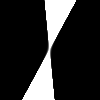
\includegraphics[width=.7\linewidth]{images/GaussianRay1.png}
        \caption{Negative Determinant}
        \label{fig:hyperbolicsub1}
      \end{subfigure}%
      \begin{subfigure}{.5\textwidth}
        \centering
        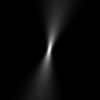
\includegraphics[width=.7\linewidth]{images/GaussianRay2.png}
        \caption{Normalised}
        \label{fig:hyperbolicsub2}
      \end{subfigure}
      \caption{A Hyperbolic Distribution Showing Laser-like normalisation}
      \label{fig:hyperbolic}
      \end{figure}
      With a single image from a camera, the only valid fact about the location of an object is that it lies somewhere within an infinite cone.


    \subsubsection{Allocating Observations to Objects}
      If multiple observations are made of multiple similar objects, the observations must be allocated to the appropriate object.

      The observations must be ranked by some metric, and sorted.  For m objects, and n observatons, this takes m*n memory.  In our low resolution computer vision pipeline, the number of visually non-unique objects is very small, and the number of objects that can be distinguished in one frame is limited by processing power.



    \subsubsection{Extensions}
      Using a vector difference of positions to estimate the velocity, models of objects can be evolved over time and updated with additional measurements.  With additional statistical analysis, this can be extended to a form consistent with Kalman style filter for the motion of every visible landmark.

      Storing a motion history of the objects would facilitate the generation of a time-dependent network of estimated locations and relative measurements.
      Here, the nodes represent the instantaneous locations of the objects, linked forward in time by velocity estimates, and linked in space by relative distance measurements.  Assumptions can be added to this mix in the same form as the object locations, time evolution and relative measurements.  A live process need only deal with the instantaneous positions of the robot and landmarks, but the models can be further refined less-than-live by a graph traversal.
      A SLAM process can be initialised by an assumption in the form of an artificial survey marker at boot. The assumptions can be later removed and replaced by real survey markers, with the map fully regenerated by the graph traversal process which need not be on-board the robot.
      
      Some computer vision processes like optical flow are able to resolve velocity coupled to depth.
      As it stands, the uncertainty analysis on our platform does not account for correlations between velocity and position, but the matrices can simply be expanded to six dimensions.
      XXX See control system theory, state vectors and time-step matrices.

  \subsection{Current implementation}
    \subsubsection{Strengths}
      
      Encodes appropriate information in a covariance matrix form
      As it stands, all data relating to external objects is fed into the object tracking routine in a covariance matrix format.  

      These covariance matrix forms mix cleanly 
      Cleanly integrates multiple observations into an object model

      Makes assumptions explicitly
      We have tried to make all of our assumptions explicitly, and have even begun to express them as covariance forms.
      For example, to assess the stability of the object locator, we set the observation allocator to create a new object for each observation and assumed the object was at ground level.  This assumption was in the same covariance model format as any other observation in the system; this time, a singular matrix defining an infinite plane at zero altitude.


    \subsubsection{Weaknesses}
      At the moment, the observation models do not account for angular uncertainties at all.  In particular this creates problems with pitch and roll compensation for the body and gimbal of the copter.
      At the moment, the camera data is assumed to have a columnar uncertainty distribution which is clearly false.  from there, the ray is rotated by several matrices representing the roll, pitch and yaw of the copter and the gimbal.  Neither of these matrices serve to encode additional angular uncertainties into the observation.
      The uncertainty in the rotation of the body of the copter is quite well known by the flight computer, but the time of arrival of the messages encoding pose has some uncertainty.  Along with the high angular velocities from the aggressive control loops, this temporal uncertainty can introduce significant angular uncertainty.

      Consistent treatment of rotational uncertainties between coordinate systems would be best represented by chains of relative uncertainties in a graph traversal type SLAM system.  In our case, this would allow the lidar and the camera to have a small relative angular uncertainty between them from by merit of being mounted on the same gimbal.

      GPS drift has been deliberately assumed to be negligible, with its effects compensated by assuming a high velocity uncertainty on all detected objects.  This way, the system will operate based on effectively DGPS resolution which is the case on all current chase-cam implementations anyway.

      The assumption that the statistics of measurement follow a Gaussian distribution requires that the measurements be unbiased.  For the angular measurements, this introduces stringent requirements for calibration which have not yet been met satisfactorially.  In particular, the servo driven camera gimbal is the single greatest source of error, being mechanically fragile and in need of frequent repair and recalibration, and also seeming to have its zero position drift between every flight.

      The Gaussian statistics is also not capable of describing complex distributions.  Some of the best examples of advanced uncertainty treatment come out of high energy physics.  In many cases, the uncertainty distributions are encoded in a rastered probability density function, or a Fourier series with effectively unbounded order.  Such advanced treatment is undoubtedly beyond the computing capacity of commodity UAVs, but a middle ground of complexity can probably be found by mixing the above Gaussian treatment with some of the statistical weighting features of Kalman style models that also solve for sensor biases.

        (image: arbitrary geometry Uncertainty Images from SoggyDog)

      


\section{Test Results}

  \subsection{Simulation tests}
    We used the simulator built alongside the arducopter firmware to run our tests.  This simulator is detailed enough to handle the inertial model of the platform and inject noise into the sensors.
    This simulator allows us to run our full software stack on any computer with a functioning compiler.
    The object tracking code estimates the location of the objects using data from the camera and flight controller covering the gimbal pose, the roll, pitch and yaw of the copter, and the GPS location as fused with the accelerometer and gyro data.

    Because the the camera cannot resolve range, an assumption model describing the ground was added to the code reducing the columnar vision model to a spot on the ground.

    Using a servo driven gimbal on the real copter we cannot perform mechanical compensation of the pitch and roll without injecting extremely large angular uncertainties.
    The object estimation code compensates for the pitch and roll using matrices representing body rotations under OpenCV.
    This compensation is designed to cleanly counter the non-linear second order signal injection, but with the camera mechanically coupled to a laptop instead of the simulated copter, the loop becomes completely unstable.

    Commenting out the pitch and roll decoupling code makes the copter very well-behaved in the simulator, using a pose generator that attempts to place the object at a ray cast forward and down from the copter, the copter can be confidently led around the simulation environment.  If the object appears behind the copter, the copter moves away from the object, turning around as it does so.

    Associating observations with objects 


  \subsection{Live tests}
    The observation allocation routine selects the most likely object an observation could refer to. If the associated probability is below some threshold, it instead creates a new object.
    In one of the tests, velocity predictions were enabled along with object creation with an inverted axis on the inertial compensation matrices. This system quickly generated more than seventy unique objects in memory and ran velocity prediction on all of them live. The algorithm's CPU usage never approached the requirements for the computer vision despite running an unoptimised sorting and allocation routine, and uncertainty analysis.
    

    The copter is able to physically follow one object, while tracking multiple others, though maintaining calibration on multiple systems has severely limited the opportunities for testing edge cases.

    The change from RC inputs to Velocity vector commands for the sake of control linearity resulted in much more predictable and consistent behaviour without significant loss of control bandwidth.
    To reduce the length of the feedback loop, we used the guided waypoint functions and absolute yaw commands in Arducopter 3.x.  This change drastically improved the flight stability of the copter, but significantly reduced the control bandwidth.  The waypoint updates appear to to be obeyed at several Hertz, despite a new request being sent every frame (30Hz).

    Basic colour matching limitations, false positives
    The feature detection algorithm used in all testing of this platform was very simple colour space thresholding.  In uncontrolled environments, this results in multiple detected features with no effective means of differentiating them.  The uncertainty analysis did appear to help with this in the limited live testing it received, but the code was not sufficiently ready to draw any generalised conclusions.

    Many more advanced object detection processes became available on our platform over the course of the project thanks to the work of Tan \cite{Tan}, but these were in active development throughout the project and offered no consistent foundation to test upon.

    As mentioned earlier, the Arducopter firmwares offer a GPS driven \"follow me\" mode using the Android application \"Tower\".  
    Our Computer vision only routines are by no means as robust as radio links and DGPS and greatly increase the complexity of the system, but the computer vision allows controlled pose and framing, and functions in urban canyon environments.

\section{Future Work}

  The UWA hexacopter platform is beginning to reach a level of hardware maturity where work can be focussed on new algorithms and applications.  Key improvements yet to be made relate to the gimbal and camera.

  The gimbal can be greatly improved by simply removing the gimbal entirely in favour of a fixed camera mount, or swapping the existing servo driven gimbal out for a Brushless DC motor driven gimbal for accurate mechanical image stabilisation.  The camera could benefit from a wider angle lens, however, the narrow field of view did prompt us to find a sound solution to tracking an object beyond the frame boundary.

  As discussed in \ref{sec:hyperbolicCase}, the uncertainty analyses are incomplete.  Further exploration of the hyperbolic case and singular matrices would permit the use of Kalman style path prediction and improve the tracking stability.
  Without solutions to the hyperbolic uncertainty case or rotational transforms, the object tracker will have somewhat unpredictable accuracy.  However, the system does function and can still benefit from case-specific functions to generate camera angles to suit artistic direction.

  Handling the velocity of external objects is not quite usable yet, though the code base does contain most of the requisite functions.  The code that extrapolates object object position based on velocity has been largely disabled, pending live tests of the more advanced observation allocation algorithms.  Until the objects' positions are being updated and adjusted live, there will be no data to infer velocity from, so the velocity handlers will simply be place-holders to maintain the size of the positional uncertainty of the objects.

  SIFT algorithm
  A problem addressed in \ref{sec:objectAllocation} is that the objects detected by colour thresholding have a non-zero size which goes against the assumptions implicit in the statistical treatment of the observations.  Using an algorithm like SIFT would track multiple points on any given object, and provide nearly unique visual identifiers for allocating observations to individual objects.  While this would eliminate a small sorting routine in the object allocator, the overheads of SIFT may well require a larger computing budget.

  Optical Flow
  Optical Flow is an extremely interesting avenue of research for small UAVs because the high compute-cost can be handled by dedicated silicon like an FPGA.  Coupled with a covariance uncertainty analysis, Optical flow is able to resolve the relationship between relative velocity and proximity between copter and object with every frame from the camera.  

  Adding a stereo pair of cameras to the copter using the large 550mm base-line afforded by the frame, would create multiple simultaneous position and velocity measurements, eliminating the Z-axis ambiguity over a significant usable range.  
  Using data from stereo image sources is well solved by our existing uncertainty analysis, though the camera input options are limited on the RPi. I would strongly recommend the inclusion of a vision co-processor to handle frame synchronisation if Stereo imaging is explored.  This vision co-processor could also accelerate edge-detection and optical flow processes.

  The current structure of the code base is sound, but makes it difficult to run processes like object tracking and object avoidance simultaneously.  This situation could be improved by using a subscriber model between different processes, such as that used by ROS.

  When we started with the new flight controller, we were using the Arducopter 3.2 firmware. To exploit new gimbal features for the object tracker, we upgraded to Arducopter 3.3rc10 and finally 3.3 stable when it released near the end of the project.  The next version of the firmware is set to include features like guided-mode without a GPS lock requirement, which will open possibilities for fully computer vision driven algorithms.  The UWA platform will continue to benefit from improvements to the Arducopter firmware into the foreseeable future.

\section{Conclusions}
  We have greatly improved the capabilities of the UWA autonomous hexacopter platform, and have brought the code-base up to a level where it is feasible to implement rudimentary SLAM processes.
  We have also demonstrated that low-power single board computers can perform live computer vision processes and rudimentary SLAM processes with uncertainty based reasoning to track and follow moving objects.






%Referencing
%---------------------------------------------------------
%\pagebreak
\renewcommand{\refname}{References}
\addcontentsline{toc}{section}{References}
\bibliography{references/refs}
\bibliographystyle{ieeetr}
%\addbibresource{references/refs.bib}
%\printbibliography

%---------------------------------------------------------

\begin{appendices}
  %\addcontentsline{toc}{section}{Appendices}
%  \section{ArduPilot (Pixhawk) Proposal} \label{sec:PihawkProposal}
%    \includepdf[pages=-]{../picopter/Documents2015/ardupilot-proposal/ardupilot-proposal.pdf}

\end{appendices}

  
\end{document}

